\section{Push notifications}
In our application, having push notifications is fundamental not only to remind the user that some food is expiring on the fridge but also to help communication and interactions among users belonging to the same family group. Each notification is delivered directly to all the users belonging to the same family when one of the four following actions take place:

\begin{itemize}
    \item[--] A user joins your family
    \item[--] A user adds a product
    \item[--] A user adds a shopping list
    \item[--] There are some products expiring in the current day
\end{itemize}

\subsection{Implementation}
Push notifications are centralized on Google and Apple servers for security reasons. For this reason, our application makes use of the \textbf{Firebase cloud messaging} service. This allows us to avoid implementing communication towards APNs which is all handled by Firebase making the notification service almost completely transparent to the developer.

\hspace*{-1cm}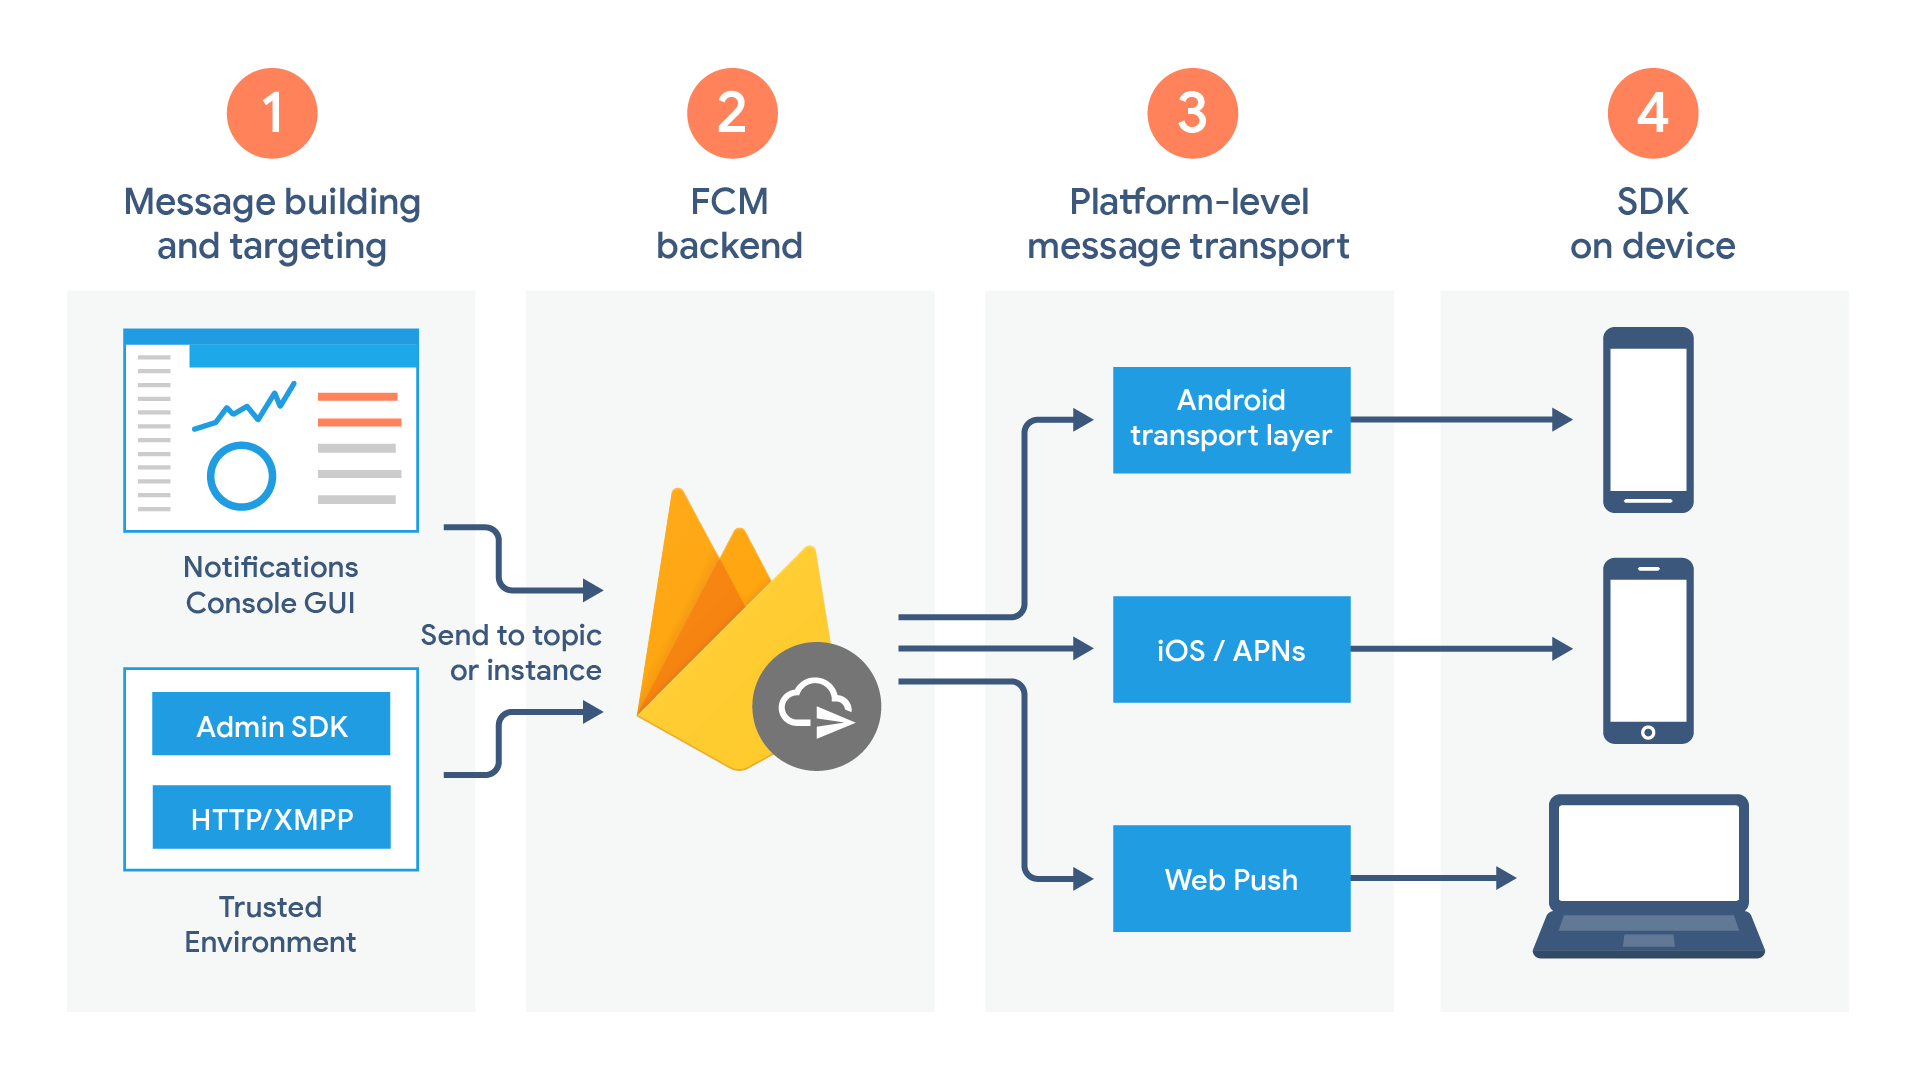
\includegraphics[width=14cm,keepaspectratio]{Images/notifications/diagram-FCM.png}

\noindent Each physical device is registered to a 'topic' which corresponds to the family id and a topic name is essentially an identifier for a pool of observers waiting for possible notifications.
\newline\newline
\noindent To sent notifications programmatically, we made use of \textit{Firebase functions}. We attached three different listeners on new additions on shopping lists, products and users. There is also a scheduled function programmed to run each day at 7a.m. and inform users is a product is expiring that day (Crontab notation).

\vspace*{0.5cm}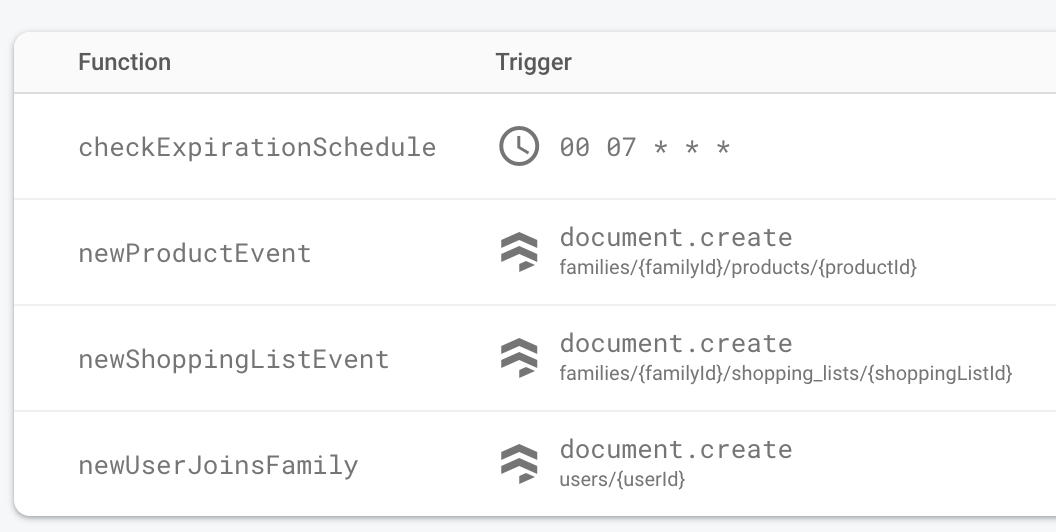
\includegraphics[width=10cm,keepaspectratio]{Images/notifications/firebase_functions.png}


\subsection{Notifications}

\begin{figure*}[h]
\begin{multicols}{2}
    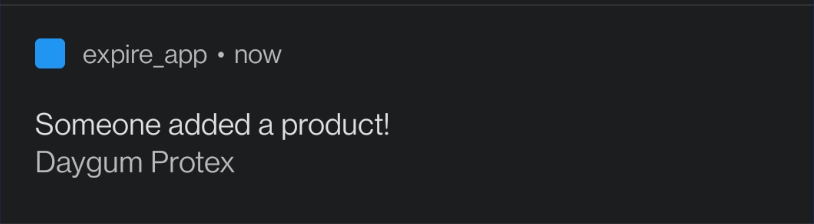
\includegraphics[width=\linewidth]{Images/notifications/new_product.png}\caption{New product added}\par 
    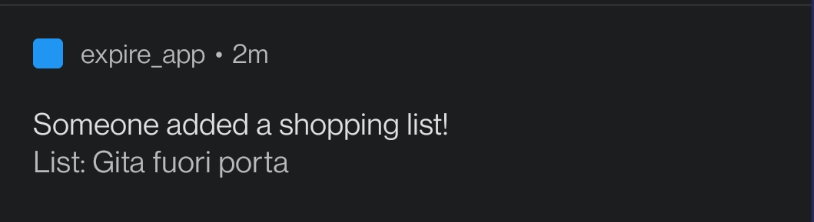
\includegraphics[width=\linewidth]{Images/notifications/new_shopping_list.png}\caption{New shopping list added}\par 
    \end{multicols}
\begin{multicols}{2}
    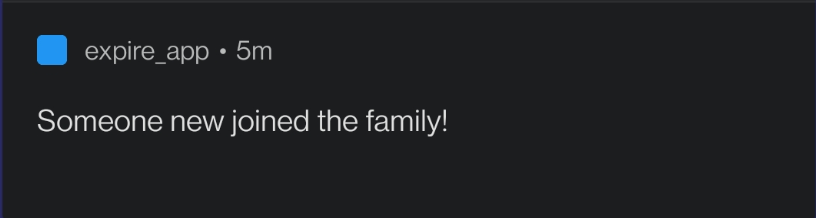
\includegraphics[width=\linewidth]{Images/notifications/new_user_family.png}\caption{New family join}\par
    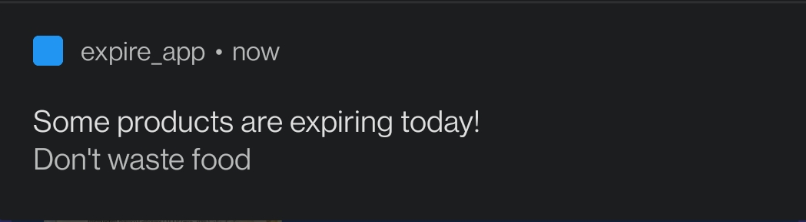
\includegraphics[width=\linewidth]{Images/notifications/expiring_notification.png}\caption{Expiration reminder}\par
\end{multicols}
\end{figure*}

Each notification is attached to its corespondent listener (Firebase trigger function) \textit{onCreate}.
\newline
\newline
\noindent\textbf{New product}
\begin{lstlisting}[caption=My Javascript Example]
exports.newProductEvent = functions.firestore
    .document("families/{familyId}/products/{productId}")
    .onCreate((snap, context) => { ... }
\end{lstlisting}
\newline
\noindent\textbf{New shopping list}
\begin{lstlisting}[caption=My Javascript Example]
exports.newShoppingListEvent = functions.firestore
    .document("families/{familyId}/shopping_lists/{shoppingListId}")
    .onCreate((snap, context) => { ... }
\end{lstlisting}
\newline
\noindent\textbf{New user joins family}
\begin{lstlisting}[caption=My Javascript Example]
exports.newUserJoinsFamily = functions.firestore
    .document("users/{userId}")
    .onCreate((snap, context) => { ... }
\end{lstlisting}

\newline
\noindent\textbf{Scheduled timer for recurrent notification}
\begin{lstlisting}[caption=My Javascript Example]
exports.checkExpirationSchedule = functions.pubsub.schedule("00 07 * * *")
    .timeZone("Europe/Rome")
    .onRun(async (context) => { ... }
\end{lstlisting}